\section{问题四：技术演进分析与能力前沿预测}
\label{sec:problem4}

\subsection{口径界定与数据准备}

\subsubsection{四项口径}

\begin{enumerate}
\item \textbf{综合能力的度量。}采用 Open LLM Leaderboard v2\cite{fourrier2024openllm} 的六项官方归一化得分（IFEval、BBH、MATH Lvl 5、GPQA、MuSR、MMLU-PRO）的算术平均
\begin{equation}
S_i=\frac16\sum_{k=1}^{6}S_{ik},\qquad S_{ik}\in[0,100],
\label{eq:p4_S}
\end{equation}
其中各项已按官方规则扣除随机猜测下界\cite{huggingface2024normalization}。复算结果与官方 Average 的最大绝对误差为 $1.4\times10^{-14}$。选用等权平均的理由是：六项任务覆盖指令遵循、推理、数学、专业知识与多步推理，等权可避免人为偏好；作为敏感性分析，另构造六维秩正态平衡分。
\item \textbf{开源筛选口径。}入选模型须在 C2 或高置信 C4 记录中有\textbf{开放权重}证据；严格敏感性分析进一步要求许可证允许研究与复现（许可证缺失不视为无限制）。闭源模型与仅开放 API 的模型不入选。
\item \textbf{模型类型。}区分 pretrained（预训练基础模型）、posttrained（chat/finetuned，经对话指令或监督微调）、merge（权重合并）与 excluded。\textbf{贡献分解只使用 pretrained 及持续预训练模型}，以免把微调收益或基座算力重复计入预训练规模；posttrained 层只有 6 条合格算力记录，不足以独立分解，仅作覆盖说明。
\item \textbf{时间轴口径。}主分析按排行榜\textbf{提交日期}计时（有效范围 2024-06-08 至 2025-03-13），因为它对所有记录统一可得；以模型发布日期作为敏感性分析。
\end{enumerate}

\subsubsection{数据清洗与证据分层}

数据使用方式见表~\ref{tab:p4_data}，清洗与复现结果见图~\ref{fig:p4_data}。

\begin{table}[htbp]
\centering
\small
\caption{问题四的数据与用途}
\label{tab:p4_data}
\begin{tabular}{p{0.10\linewidth}p{0.24\linewidth}p{0.56\linewidth}}
\toprule
数据 & 规模 & 用途与处理 \\
\midrule
C1 / C2 & 4576 条，版本去重后 4546 条 & 六任务能力、提交日期、模型类型与许可证；C2 为主表，C1 核验分数 \\
C3 & 26 条论文/报告记录 & 2023--2024 长窗口的方向性检验 \\
C4 & 3523 条，接受匹配 66 条 & 训练算力、数据量、开放权重证据；按名称、组织、族、版本、参数量五项匹配，最终 41 条进入确认性前沿（7 个月、13 个模型族） \\
C5 / C6 & 43 / 75 条 & Loss--Benchmark 桥接（C5 为 C6 子集，只用 C6 拟合一次） \\
C7 & 45 条 & 上下文长度可行取值（问题三） \\
C8 & 1863 个模型目录 & 逐任务重算：BBH 子任务聚合 \\
\bottomrule
\end{tabular}
\end{table}

\begin{figure}[htbp]
\centering
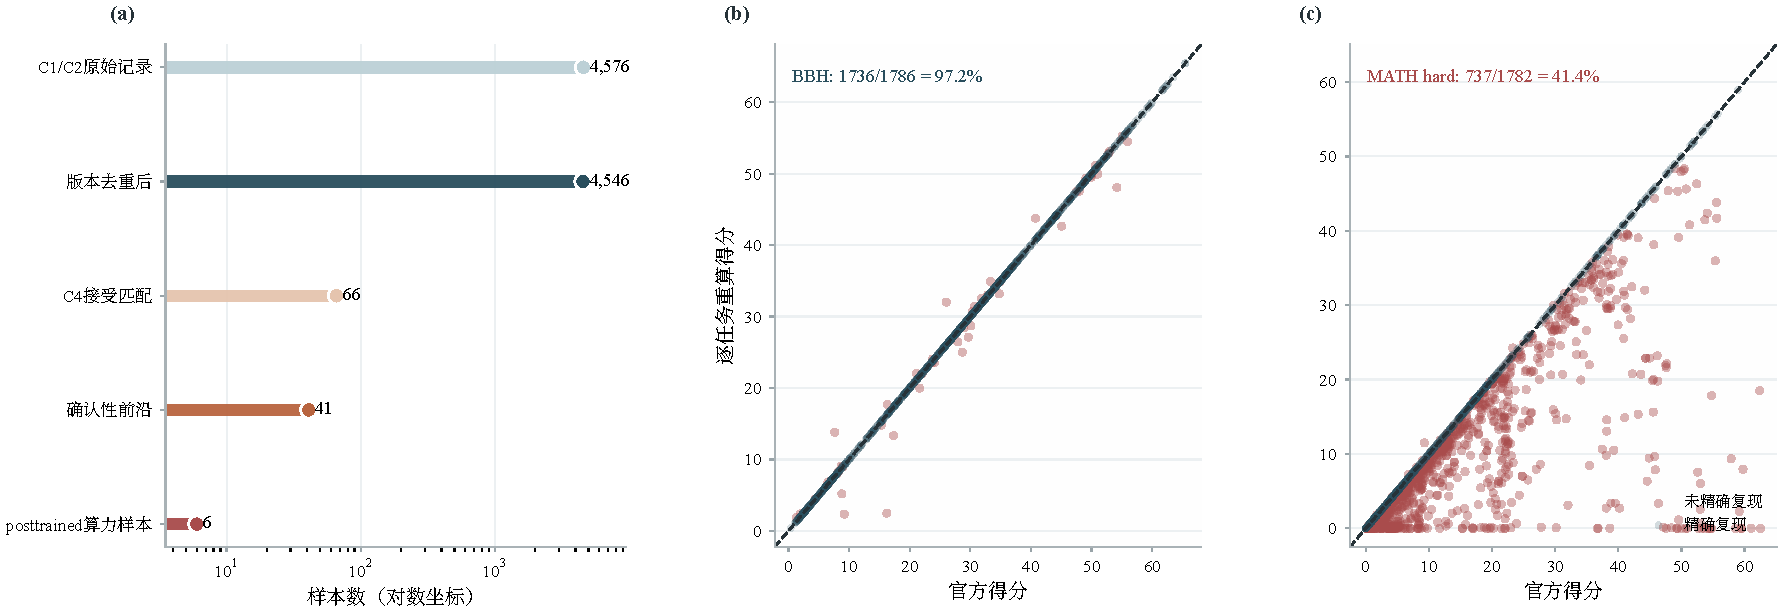
\includegraphics[width=\linewidth]{images/no4/P4_F01_数据筛选与逐任务复现审计.pdf}
\caption{数据筛选过程（a）与 C8 逐任务重算：BBH（b）、MATH Lvl 5（c）}
\label{fig:p4_data}
\end{figure}

\textbf{C8 逐任务聚合分析。}按官方规则，BBH 的每个子任务先扣除随机猜测下界再等权平均：
\begin{equation}
z_{ij}=\max\left\{0,\ \frac{s_{ij}-l_j}{1-l_j}\right\},\qquad \widehat S_i^{\mathrm{BBH}}=\frac{100}{|J_i|}\sum_{j\in J_i}z_{ij},
\label{eq:p4_bbh}
\end{equation}
其中 $s_{ij}$ 为模型 $i$ 在子任务 $j$ 上的原始准确率，$l_j$ 为随机下界。在 1786 个可比模型中，重算值与官方值精确一致的有 1736 个（$97.2\%$），证明汇总表的 BBH 得分可由逐任务数据复现。MATH Lvl 5 仅 737/1782 精确一致，且偏差系统性地位于对角线下方，推测官方聚合使用了未公开的子集过滤规则，故 MATH 的逐任务结果只作审计参考，不影响式~\eqref{eq:p4_S} 的主表。

\subsection{Loss--Benchmark 桥接模型}

\subsubsection{模型形式}

Loss 与下游能力总体负相关，但二者并非一一对应：相同预训练 Loss 可能对应不同的下游能力\cite{liu2023samepretraining}，离散的评测指标还会放大或掩盖连续的 Loss 变化\cite{schaeffer2023emergent,du2024understanding}。为保证预测落在 $[0,100]$，先作有界 logit 变换
\begin{equation}
g_\epsilon(S)=\operatorname{logit}\frac{S+\epsilon}{100+2\epsilon},\qquad g_\epsilon^{-1}(y)=(100+2\epsilon)\sigma(y)-\epsilon,\qquad \epsilon=0.5,
\label{eq:p4_link}
\end{equation}
再建立单调桥接
\begin{equation}
g_\epsilon(S_{im})=h_m(\ln L_i)+e_{im},\qquad h_m'(\cdot)\le0,
\label{eq:p4_bridge}
\end{equation}
$h_m$ 在常数、单调线性、单调样条、保序回归四类候选中选择。C6 按可比性分级：高可比记录权重为 1，中可比记录权重为 0.25。以\textbf{来源族留一}交叉验证（12 个来源族）评价，按一倍标准误原则选最简模型。

\subsubsection{选择结果}

\begin{figure}[htbp]
\centering
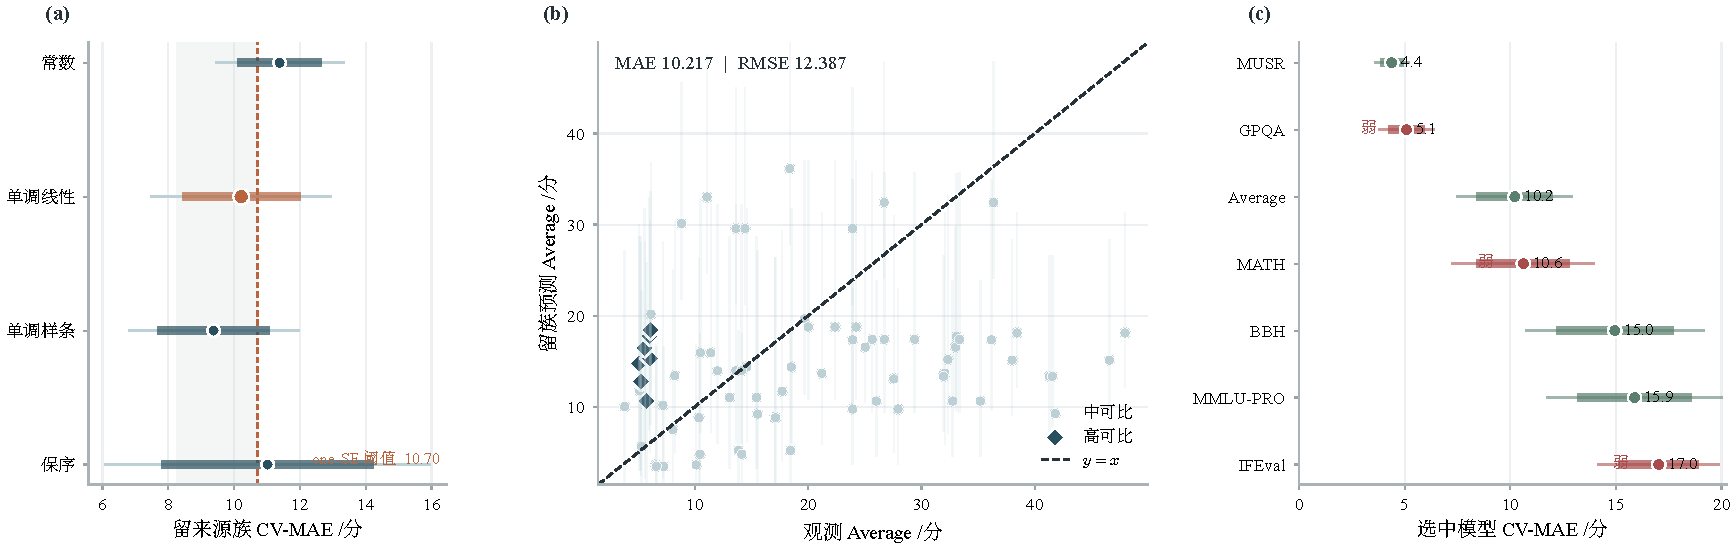
\includegraphics[width=\linewidth]{images/no4/P4_F02_Loss_Benchmark桥接选择与留族验证.pdf}
\caption{Loss--Benchmark 桥接：候选模型比较（a）、Average 留族预测（b）与七类目标的桥接误差（c）}
\label{fig:p4_bridge}
\end{figure}

结果见图~\ref{fig:p4_bridge}。对综合能力 Average，单调样条的留族 MAE 最低（$9.38$），单调线性为 $10.22$，落在一倍标准误阈值（$10.70$）以内，故选择更简单的单调线性桥接；它优于常数基线（$11.38$），RMSE 为 $12.39$。在六项子任务中，BBH、MuSR、MMLU-PRO 的桥接优于常数基线，IFEval、MATH、GPQA 则未能稳定优于常数，说明\textbf{指令遵循与高难度数学、专业问答能力不能由预训练 Loss 可靠预测}，这与 Loss 之外的后训练因素主导这类能力的认识一致\cite{ruan2024observational,schaeffer2025predicting}。因此只用 Average 承担主结论。桥接的完整支持区间为 Loss $\in[1.65,2.84]$，其中高可比范围为 $[2.093,2.598]$。

\subsubsection{问题三方案的能力映射与误差影响}

\begin{figure}[htbp]
\centering
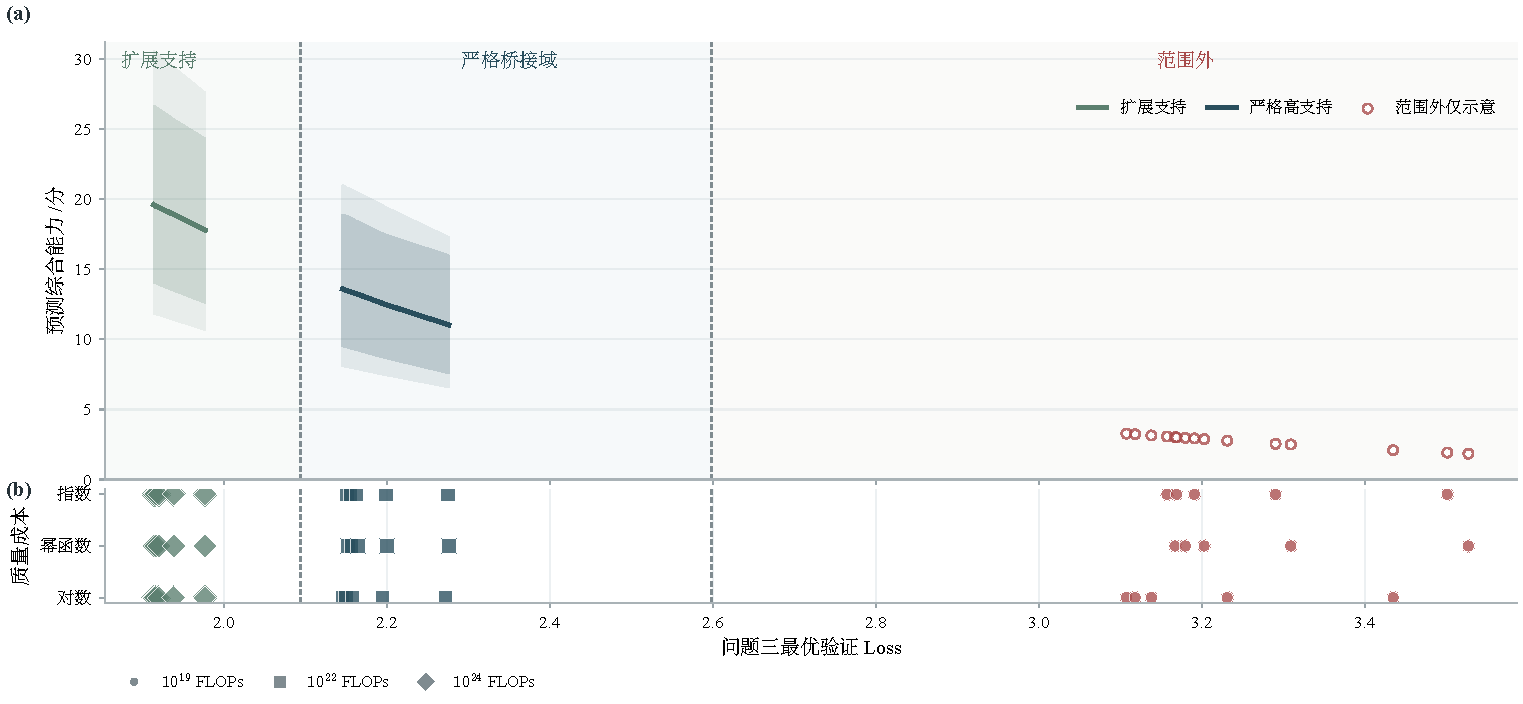
\includegraphics[width=0.94\linewidth]{images/no4/P4_F03_问题三Loss到综合能力映射.pdf}
\caption{问题三 45 个最优方案的 Loss 到综合能力映射及桥接支持区间}
\label{fig:p4_map}
\end{figure}

\begin{table}[htbp]
\centering
\small
\caption{$L_{\mathrm{ctx}}=4096$ 下问题三最优方案的能力映射（参考配比）}
\label{tab:p4_map}
\begin{tabular}{llcccl}
\toprule
质量成本 & 预算/FLOPs & 最优 Loss & 能力中位数 & 80\% 区间 & 桥接支持 \\
\midrule
指数 & $10^{19}$ & 3.169 & 3.00 & [1.68, 6.26] & 范围外 \\
 & $10^{22}$ & 2.155 & 13.39 & [9.37, 18.68] & 高可比 \\
 & $10^{24}$ & 1.916 & 19.51 & [14.02, 26.56] & 扩展支持 \\
\midrule
幂函数 & $10^{19}$ & 3.180 & 2.97 & [1.63, 6.24] & 范围外 \\
 & $10^{22}$ & 2.156 & 13.36 & [9.35, 18.63] & 高可比 \\
 & $10^{24}$ & 1.916 & 19.51 & [14.02, 26.56] & 扩展支持 \\
\midrule
对数 & $10^{19}$ & 3.118 & 3.22 & [1.83, 6.63] & 范围外 \\
 & $10^{22}$ & 2.150 & 13.49 & [9.46, 18.80] & 高可比 \\
 & $10^{24}$ & 1.916 & 19.52 & [14.03, 26.57] & 扩展支持 \\
\bottomrule
\end{tabular}
\end{table}

结果见表~\ref{tab:p4_map} 与图~\ref{fig:p4_map}。三种成本函数在中高预算下的映射能力几乎相同（差异 $<0.2$ 分），与问题三“高预算下成本形状不再重要”一致。预算每提高两个数量级（$10^{22}\to10^{24}$），综合能力约提高 $6$ 分。若采用近优配比 $\boldsymbol p^\star$，按中心桥接换算，$10^{22}$、$10^{24}$ FLOPs 的综合能力约可再提高 $1.9$ 分和 $1.3$ 分。

\textbf{映射误差的影响。}把问题三的 Loss 抽样与桥接的来源族 bootstrap 配对传播，得到三组区间宽度（图~\ref{fig:p4_bt}(b)）：仅上游 Loss 不确定性的 $80\%$ 宽度中位数约为 $0.00$ 分（最大 $0.09$），仅桥接不确定性为 $9.17$ 分，联合为 $9.17$ 分。\textbf{映射误差是能力结论不确定性的绝对主导来源}，比优化器与标度律参数误差大两个数量级。因此：（1）能力的\textbf{相对比较}（不同成本、不同预算之间）是可靠的，因为同一桥接的误差高度正相关；（2）能力的\textbf{绝对水平}只能以约 $\pm5$ 分的精度解读；（3）低预算方案的 Loss（$>3.1$）超出桥接支持上界，其能力值仅作量级参考。

\subsection{能力前沿的动力学模型}

\subsubsection{条件分位前沿}

能力前沿关心的是“给定算力与时点，较优的模型能达到多高”，而不是平均水平，因此采用 $\tau=0.90$ 条件分位回归\cite{koenker1978quantiles}。令 $Y_i=g_\epsilon(S_i)$，$x_i=\log_{10}C_i$（训练算力，标准化为 $\tilde x_i$），建立
\begin{equation}
Q_\tau(Y_i\mid x_i,t_i)=\beta_0+\beta_C\tilde x_i+a_{m(i)},\qquad \beta_C\ge0,
\label{eq:p4_frontier}
\end{equation}
其中 $a_m$ 为提交月份 $m$ 的\textbf{非规模技术状态}，吸收架构、数据工程、优化方法等不随算力度量的因素。主模型只放入训练算力 $C$，而不同时放入 $N$ 与 $D$，以避免 $C\approx6ND$ 引起的机械共线。

\subsubsection{技术状态的动力学方程}

技术状态按局部线性趋势演进\cite{hyndman2021forecasting}：
\begin{equation}
a_m=a_{m-1}+v_{m-1}+\eta_m,\qquad v_m=v_{m-1}+\zeta_m,
\label{eq:p4_state}
\end{equation}
$v_m$ 为技术进步速度。数值上以平滑 pinball 损失加一阶、二阶差分惩罚实现，平滑强度 $\lambda$ 与未来斜率权重 $\rho$ 只由 3、6 个月滚动起点回测选择（每一折只用预测时点以前的数据）。最终 $\lambda=10^4$、$\rho=0$，标准化算力系数 $\widehat\beta_C=0.685>0$。三条分位（$0.85,0.90,0.95$）若交叉，则单调重排\cite{chernozhukov2010quantile}。

\begin{figure}[htbp]
\centering
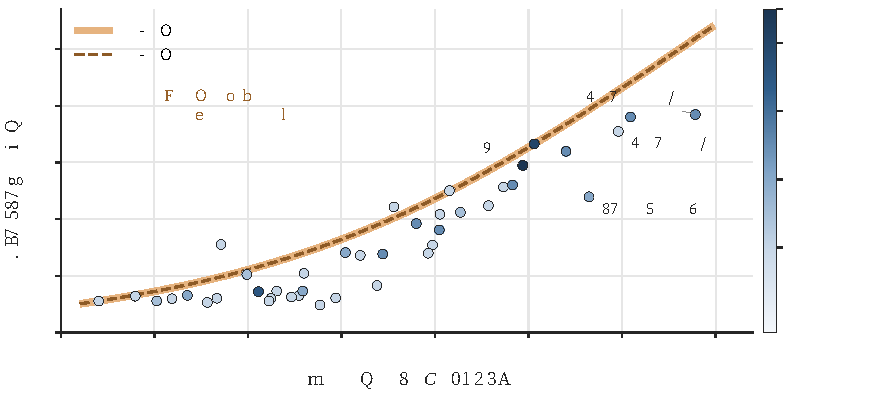
\includegraphics[width=0.94\linewidth]{images/no4/P4_F04_训练算力与动力学能力前沿.pdf}
\caption{确认性 pretrained 样本的训练算力与 $0.90$ 能力前沿（2024-06 与 2025-01）}
\label{fig:p4_front}
\end{figure}

图~\ref{fig:p4_front} 显示，能力前沿随训练算力呈清晰的上凸增长：在 $\log_{10}C$ 从 $21.6$ 增至 $25.0$ 的范围内，前沿由约 $5$ 分升至约 $54$ 分；观测最高分为 Qwen2.5-72B 的 $38.4$ 分（$7.8\times10^{24}$ FLOPs）。2024-06 与 2025-01 两条前沿曲线几乎重合（最大差 $0.0002$ 分），这已经直观地预示了下一节的分解结论。

\subsection{规模扩张与非规模技术进步的贡献分解}

\subsubsection{Shapley 分解}

取确认性面板的首末月份 $t_0=$ 2024-06、$t_1=$ 2025-01，以两月训练算力的 $0.90$ 分位 $x_0,x_1$ 代表前沿规模。记 $F(x,t)$ 为式~\eqref{eq:p4_frontier} 经逆变换后的能力分。由于模型非线性，“先换规模”与“先换时间”得到的增量不同，采用两因素 Shapley 值\cite{shapley1953value}取两条路径的平均：
\begin{align}
\Delta_{\mathrm{scale}}&=\tfrac12\big[F(x_1,t_0)-F(x_0,t_0)+F(x_1,t_1)-F(x_0,t_1)\big],\label{eq:p4_scale}\\
\Delta_{\mathrm{tech}}&=\tfrac12\big[F(x_0,t_1)-F(x_0,t_0)+F(x_1,t_1)-F(x_1,t_0)\big],\label{eq:p4_tech}
\end{align}
二者之和恰为总变化 $F(x_1,t_1)-F(x_0,t_0)$（数值闭合误差 $5.6\times10^{-17}$）。贡献占比定义为 $\Delta_{\mathrm{scale}}/(\Delta_{\mathrm{scale}}+\Delta_{\mathrm{tech}})$。不确定性以模型族为横截面簇、连续月份为时间块做联合块 bootstrap\cite{kunsch1989bootstrap}（1000 次）。

\subsubsection{分解结果}

\begin{table}[htbp]
\centering
\small
\caption{2024-06 至 2025-01 能力前沿提升的贡献分解}
\label{tab:p4_decomp}
\setlength{\tabcolsep}{4pt}
\begin{tabular}{lcccc}
\toprule
分解量 & 中心估计/分 & 80\% 区间 & 95\% 区间 & 贡献占比 \\
\midrule
能力总变化 & 4.618 & [2.842, 5.663] & [2.533, 6.686] & 100\% \\
规模扩张贡献 & 4.618 & [2.841, 5.664] & [2.533, 6.687] & $\approx100\%$ \\
非规模技术贡献 & $-0.0001$ & [$-0.0018$, 0.0037] & [$-0.0027$, 0.0053] & $\approx0\%$ \\
\bottomrule
\end{tabular}

\vspace{2pt}{\footnotesize 注：规模贡献占比的 bootstrap 95\% 区间为 $[99.88\%,\ 100.06\%]$。}
\end{table}

\begin{figure}[htbp]
\centering
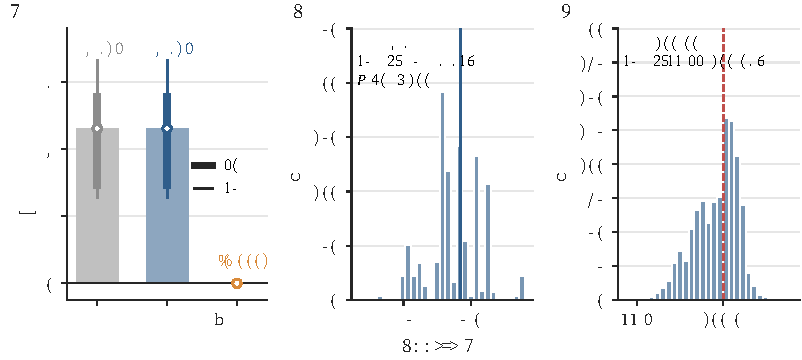
\includegraphics[width=\linewidth]{images/no4/P4_F05_规模与非规模贡献联合分布.pdf}
\caption{贡献分解的点估计与区间（a）、规模贡献（b）与规模占比（c）的 bootstrap 分布}
\label{fig:p4_decomp}
\end{figure}

由表~\ref{tab:p4_decomp} 与图~\ref{fig:p4_decomp}：2024 年 6 月至 2025 年 1 月，开源 pretrained 模型的 $0.90$ 能力前沿提升 $4.62$ 分，其中\textbf{规模扩张贡献约 100\%}（规模贡献为正的概率为 100\%），\textbf{非规模技术贡献约 0\%}，其区间在 $\pm0.005$ 分内且跨零（为正的概率 $0.53$）。

这一结论在各种设定下都稳健（图~\ref{fig:p4_sens}）：改变能力口径（平衡分）、样本边界（严格许可证、严格算力证据）、时间轴（发布日期）、边界参数 $\epsilon$ 与块长，规模贡献始终为正（$3.87$--$11.34$ 分），非规模贡献始终接近 0（除发布日期口径为 $-0.033$ 外，均在 $\pm0.0023$ 以内）。引入 C3 的 2023--2024 长窗口记录后，控制参数量后的年份系数中心为 $-0.034$、为正的概率 $0.41$，同样未检出稳定的非规模进步方向。

\begin{figure}[htbp]
\centering
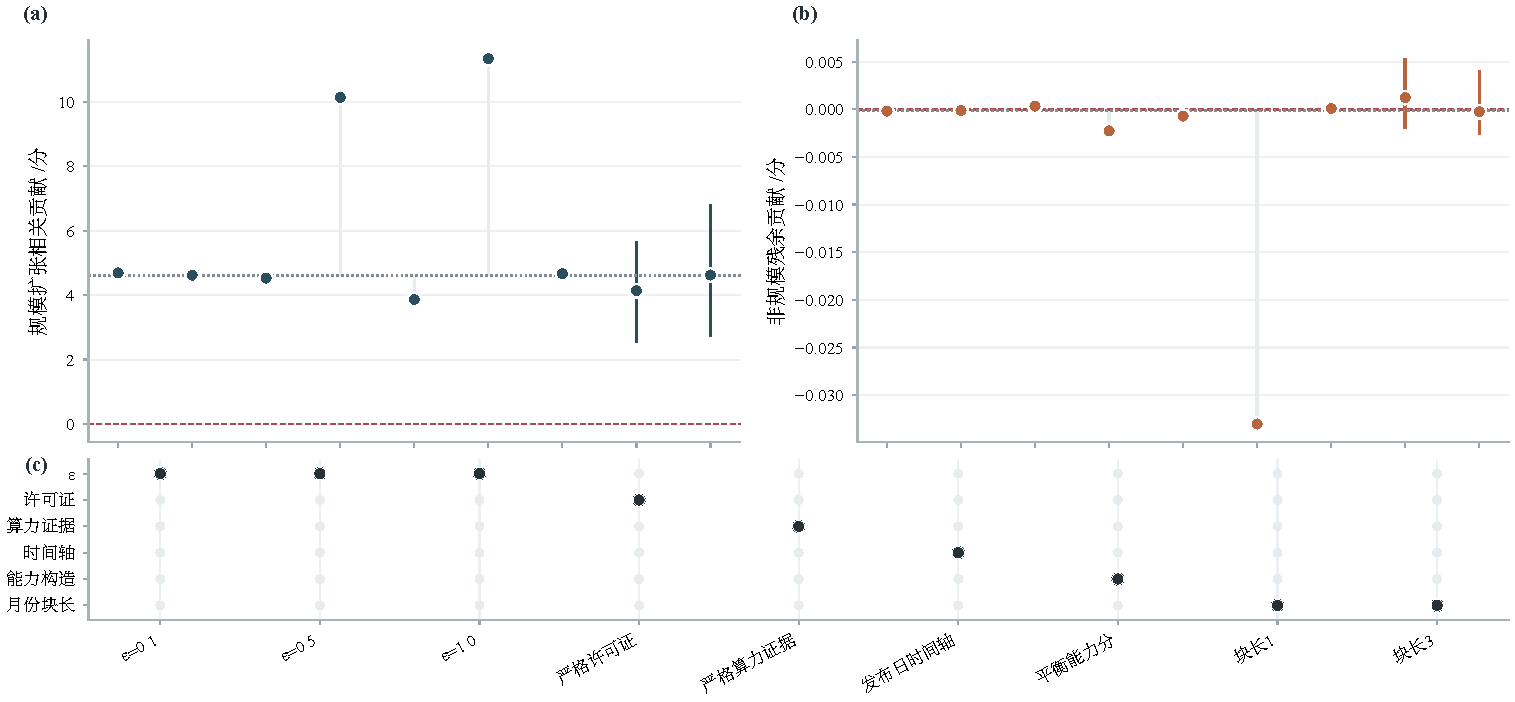
\includegraphics[width=\linewidth]{images/no4/P4_A02_贡献分解规格敏感性.pdf}
\caption{贡献分解对样本、口径、时间轴与估计参数设定的敏感性}
\label{fig:p4_sens}
\end{figure}

\textbf{如何理解“非规模贡献约为 0”。}这并不意味着架构、数据与训练方法没有进步，而是说明：\textbf{在本数据窗口内，非规模进步已经“体现”在算力—能力关系之中}，没有表现为“同等算力下能力随时间整体抬升”。有三点原因。其一，窗口只有 7 个月，而文献估计的算法进步速度约为“每 8 个月达到同等性能所需的算力减半”\cite{ho2024algorithmicprogress}，7 个月内的时间效应本就接近检测下限；其二，这一时期开源前沿模型（如 Qwen2.5 系列）的主要提升来自训练 Token 数的大幅增加，这在本文口径下计入了“规模”（$C\approx6ND$ 中的 $D$）；其三，Open LLM Leaderboard v2 的任务难度高，基础模型在 MATH、GPQA 上普遍接近随机下界，限制了非规模改进的可见度。因此，本文的分解应理解为：\textbf{近期开源基础模型的能力前沿提升几乎完全可由训练算力增长解释}。

\subsection{算力放缓情景下的能力前沿预测}

\subsubsection{算力增长趋势}

训练算力只使用截止日前、开放权重、证据方法为“直接报告、运算计数或硬件估计”的 C4 记录，由 Benchmark 反推的算力一律排除，避免循环论证\cite{epoch2025computeestimation}。对近 24 个月的家族—月份面板取加权 $0.90$ 分位，以稳健局部线性趋势得到截止月的算力端点与增速：
\begin{equation}
x_{C,0}=25.09\ \log_{10}\mathrm{FLOPs},\qquad r_C=0.759\ \log_{10}\mathrm{FLOPs}/\text{年}\ (\text{即每年}\ 5.7\ \text{倍}),
\label{eq:p4_growth}
\end{equation}
增速的 bootstrap 区间为 $[0.51,1.00]$。这与 Epoch AI 估计的前沿模型训练算力每年增长 $4$--$5$ 倍\cite{sevilla2024trainingcompute,sevilla2022compute}处于同一量级。设算力对数增速保留比例为 $\kappa$，则
\begin{equation}
x_C(h;\kappa)=x_{C,0}+\kappa\, r_C\,\frac{h}{12},\qquad \kappa\in\{1,\ 0.5,\ 0.25\},
\label{eq:p4_scen}
\end{equation}
分别代表延续近期趋势、中度放缓与强度放缓（图~\ref{fig:p4_comp}）。未来 $h$ 个月的能力前沿由式~\eqref{eq:p4_frontier}、\eqref{eq:p4_state} 与 \eqref{eq:p4_scen} 联合外推。

\begin{figure}[htbp]
\centering
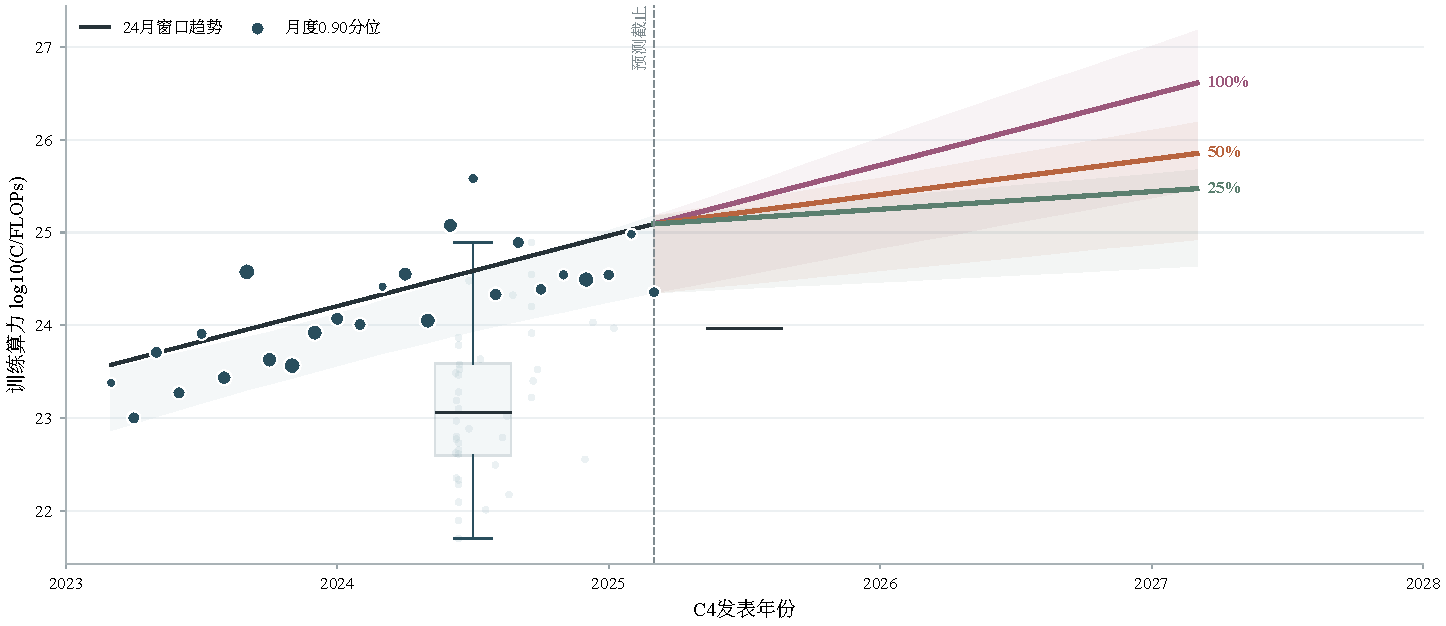
\includegraphics[width=0.94\linewidth]{images/no4/P4_F06_训练算力趋势与放缓情景.pdf}
\caption{开源模型训练算力 $0.90$ 分位的历史趋势与三种增长情景}
\label{fig:p4_comp}
\end{figure}

\subsubsection{预测结果与不确定性}

每次 bootstrap 抽样同时重估前沿参数、技术状态斜率、算力端点、算力增速与算力测量误差，1000 次抽样中 999 次有效。结果见表~\ref{tab:p4_fc} 与图~\ref{fig:p4_fc}。

\begin{table}[htbp]
\centering
\small
\caption{不同算力情景下开源模型 $0.90$ 能力前沿的预测}
\label{tab:p4_fc}
\begin{tabular}{lcccc}
\toprule
算力情景 & 预测期 & 前沿中心值/分 & 80\% 区间 & 95\% 区间 \\
\midrule
延续趋势（$\kappa=1$） & 12 个月 & 65.74 & [47.15, 78.37] & [40.25, 86.09] \\
 & 24 个月 & 77.15 & [57.30, 90.47] & [47.49, 95.29] \\
\midrule
中度放缓（$\kappa=0.5$） & 12 个月 & 59.16 & [41.91, 69.45] & [36.47, 77.85] \\
 & 24 个月 & 65.74 & [47.15, 78.36] & [40.25, 86.08] \\
\midrule
强度放缓（$\kappa=0.25$） & 12 个月 & 55.72 & [39.55, 64.64] & [34.60, 72.52] \\
 & 24 个月 & 59.16 & [41.91, 69.44] & [36.47, 77.85] \\
\bottomrule
\end{tabular}
\end{table}

\begin{figure}[htbp]
\centering
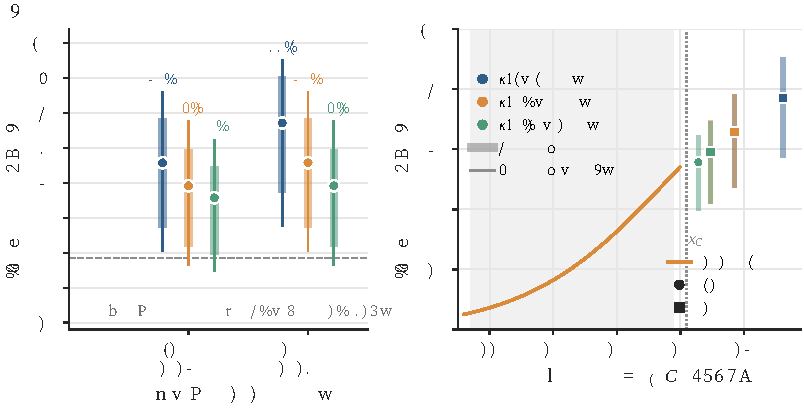
\includegraphics[width=\linewidth]{images/no4/P4_F07_算力放缓下的未来能力前沿.pdf}
\caption{不同算力情景下 12、24 个月能力前沿预测（a）及其在算力—能力前沿上的位置（b）}
\label{fig:p4_fc}
\end{figure}

\begin{enumerate}
\item \textbf{算力放缓显著压低能力前沿。}24 个月后，延续趋势情景的前沿中心值为 $77.2$ 分；若算力增速减半，降至 $65.7$ 分；若只保留四分之一，降至 $59.2$ 分。与截止时点的观测最高分 $38.4$ 相比，三种情景下 24 个月的提升幅度分别约为 $39$、$27$、$21$ 分。
\item \textbf{能力由“到达的算力”决定。}中度放缓 24 个月与延续趋势 12 个月到达相同算力（$10^{25.85}$），前沿值完全相同（$65.74$）；强度放缓 24 个月与中度放缓 12 个月亦然。这是“非规模贡献约为 0”的直接推论：\textbf{算力放缓一半，能力前沿的到达时间就推迟一倍}。
\item \textbf{不确定性较大且随期限扩大。}80\% 区间宽度约为 $25$--$33$ 分，主要来自算力增速的不确定性（$r_C$ 区间 $[0.51,1.00]$）与前沿曲线在观测范围之外的外推。12 个月预测对应的算力已超出历史观测上界，24 个月更属长期外推，预测值应结合区间使用。
\end{enumerate}

\subsection{模型检验}

\textbf{滚动回测。}在 3 个月与 6 个月步长上各设 4 个有效滚动起点，比较本文模型（M-C）与“只有时间”（M-time）、“只有规模”（M-scale）两种基线（图~\ref{fig:p4_bt}(a)）。M-C 相对 M-scale 的平均 pinball 损失差为 $0.0012$（配对标准误 $0.0012$），未劣化超过一个标准误；M-time 则明显劣于 M-scale（技能分数 $-2.08$、$-1.78$）。这再次说明\textbf{算力是能力前沿的主导解释变量，单纯的时间趋势不能替代它}。

\begin{figure}[htbp]
\centering
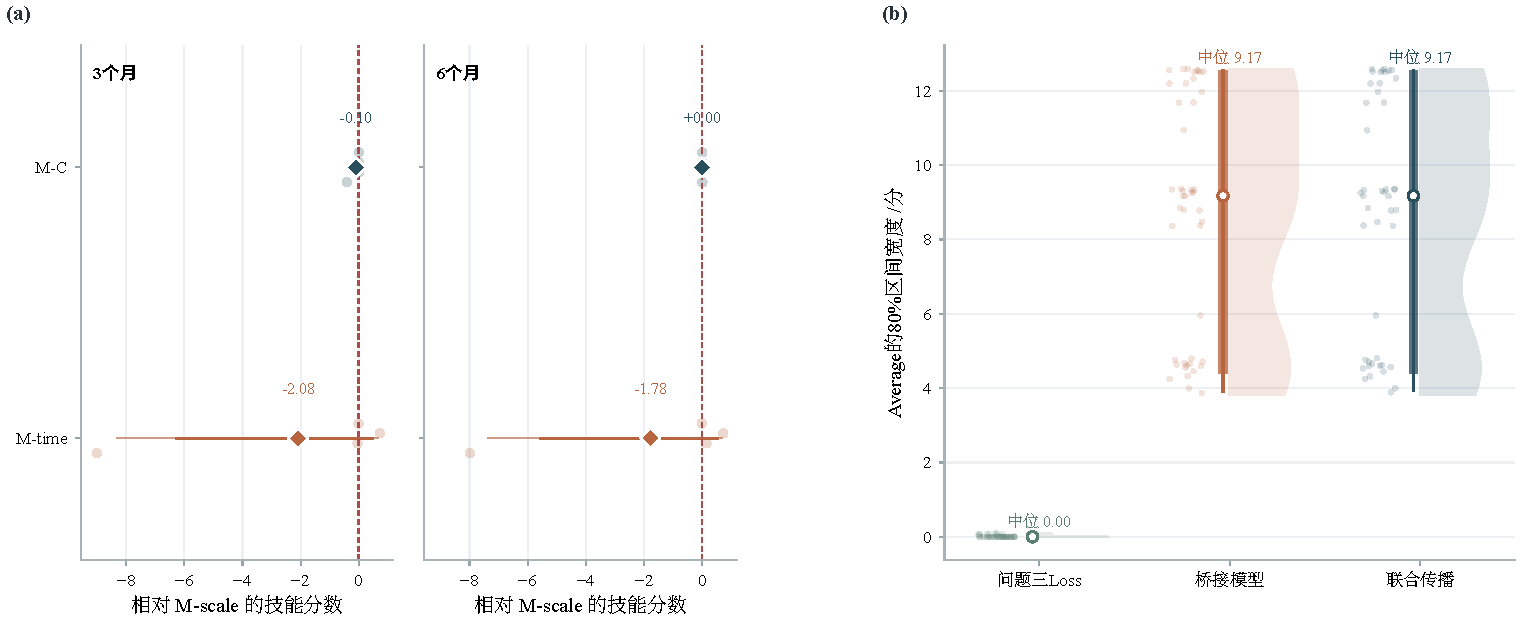
\includegraphics[width=\linewidth]{images/no4/P4_F08_滚动回测与桥接不确定性.pdf}
\caption{滚动回测的技能分数（a）与能力映射区间宽度的来源分解（b）}
\label{fig:p4_bt}
\end{figure}

\textbf{数值验证。}全部桥接在稠密 Loss 网格上无单调性违反；问题三的 45 个方案未进入历史前沿训练集；三条分位在中心预测与所有抽样中均保持有序；Shapley 分解在 logit 与得分两个尺度上闭合；相同配置重复运行结果完全一致。全部 30 项检查中 29 项通过，唯一警告为上文所述的 MATH 逐任务复现率不足，已按规则降级处理。

\subsection{问题四小结}

\begin{conclusionbox}
\textbf{问题四主要结论}
\begin{enumerate}
\item 以六项官方归一化得分的平均为综合能力，开源口径要求开放权重，贡献分解只用 pretrained 模型，时间轴取提交日期；C8 逐任务重算 BBH 的精确复现率为 $97.2\%$。
\item 单调线性 Loss--Benchmark 桥接的留族 MAE 为 $10.2$ 分；问题三的最优方案在 $10^{22}$、$10^{24}$ FLOPs 下对应综合能力约 $13.4$、$19.5$ 分。映射误差（80\% 宽度约 $9.2$ 分）是能力结论的主导不确定性来源，远大于上游 Loss 误差。
\item 2024-06 至 2025-01，开源基础模型能力前沿提升 $4.62$ 分，规模扩张贡献约 $100\%$，非规模技术贡献约 $0\%$（区间跨零），结论对口径与样本设定稳健。
\item 若算力对数增速保留 $100\%$、$50\%$、$25\%$，24 个月后 $0.90$ 能力前沿中心值分别为 $77.2$、$65.7$、$59.2$ 分（80\% 区间约 $\pm12$--$17$ 分）；算力增速减半，能力前沿的到达时间推迟一倍。
\end{enumerate}
\end{conclusionbox}
